\section{RA/Dec co-ordinate system}

We have two requirements for a co-ordinate system:
\begin{itemize}
	\item The system needs to be well defined
	\item Everyone needs to use the same one to allow for collaboration
\end{itemize}

\begin{figure}[h!]
	\centering
	\includegraphics[width=0.6\textwidth]{RaDecDrawing.png}
	\caption{Red:Ecliptic, Blue:Celestial Equator, Green:Equator}
\end{figure}

\paragraph{A Siderial Day} is the time between stars crossing the same line in
the sky. This is an absolute earth day with respect to the stars - not the Sun!
It is approx 23h56m long.

\paragraph{Example}
If a star with RA = 100$^\circ$ crosses a stationary telescope eyepiece at 11pm
and another appears in the eyepiece an hour later, what is the RA of the second
star?

Earth rotates once in 24h, so in 1h rotates $15^\circ$. Therefore the telescope
now points at first star $ + 15^\circ = 115^\circ$!

\paragraph{Example}
Two stars seen in an image:
$$
	\alpha_1 = 117.397^\circ, \; \; \delta_1 = 22.393^\circ
$$
$$
	\alpha_2 = 117.384^\circ, \; \; \delta_2 = 22.390^\circ
$$
What is the separation in arcseconds?

Because the declination difference changes depending on the RA of each, we find
that the distance is:
$$
	\Delta^2 = (\alpha_1 - \alpha_2)^2
	\cos^2\left(\frac{\delta_1 + \delta_2}{2}\right) + 
	(\delta_1 - \delta_2)^2
$$
This gives us the distance $\Delta = 44.5$ as.

\section{Fluxes and Magnitudes}

Flux is luminosity corrected for distance:
$$
	F = \frac{1}{L}(4\pi r^2)
$$
We define magnitude as a relative scale that is dependent on the fluxes of two
objects. Normally, Vega is taken as the standard.
$$
	m_a - m_b = -2.5\log\left(\frac{F_a}{F_b}\right)
$$
With the naked eye, it is possible to see a maximum of 6th magnitude stars.

\paragraph{Example}
The star RR-Lyrae ranges in magnitude from 7.1 to 7.8 in 8 hours. What is the
relative increase in brightess?
$$
	m_1 - m_2 = -2.5\log\left(\frac{F_a}{F_b}\right)
$$
$$
	10^{2.5(m_2 - m_1)} = \frac{F_1}{F_2} = 1.91
$$

\paragraph{Example}
A binary star comprises two stars, a and b, with a brightness ratio of 2. We see
them as unresolved, and the total magnitude is 5. What is the magnitude of each
star?

Let's begin by pretending we have a reference star with flux $F_0$ and magnitude
0. We also know that the fluxes of the stars sum to make the flux of the binary
system.
$$
	m_{a+b} - 0 = -2.5\log\left(\frac{F_a + F_b}{F_0}\right)
$$
Now, we can find $F_0$ in terms of the fluxes of the stars using $m_{a+b} = 5$:
$$
	100(F_a + F_b) = F_0
$$
Again using the magnitude equation, we find $m_a$:
$$
	m_a - 0 = -2.5\log\left(\frac{F_a}{F_0}\right)
$$
Substituting in:
$$
	m_a = -2.5\log\left(\frac{1}{100(1+\frac{F_b}{F_a})}\right) = 5.44
$$
We repeat for $m_b = 6.19$.

\subsection{Absolute magnitude}
Asbolute magnitude ($M$) is found by 'placing' the stars 10 pc away and
'measuring' it's magnitude. We do this mathematically with:
$$
	M = m + 5\left(1 + \log\left(\frac{d}{10}\right)\right)
$$
